\documentclass{article}
\usepackage{color}
\usepackage{amsxtra}   
\usepackage{amsthm}
\usepackage{amssymb}
\usepackage{amsfonts}
\usepackage{graphicx}   
\usepackage{rotating}

\begin{document}

\section{Supplement Materials}


\subsection{Monte Carlo Simulation}
\label{sub:MCS}
The 1D simulation is performed using Monte Carlo algorithm under the particle
scenario. The analogy of 1D polymer loop to the Fermions particle system is
shown in Figure. \ref{fig:s1}. 
\begin{figure}[htpb]
	\centering
	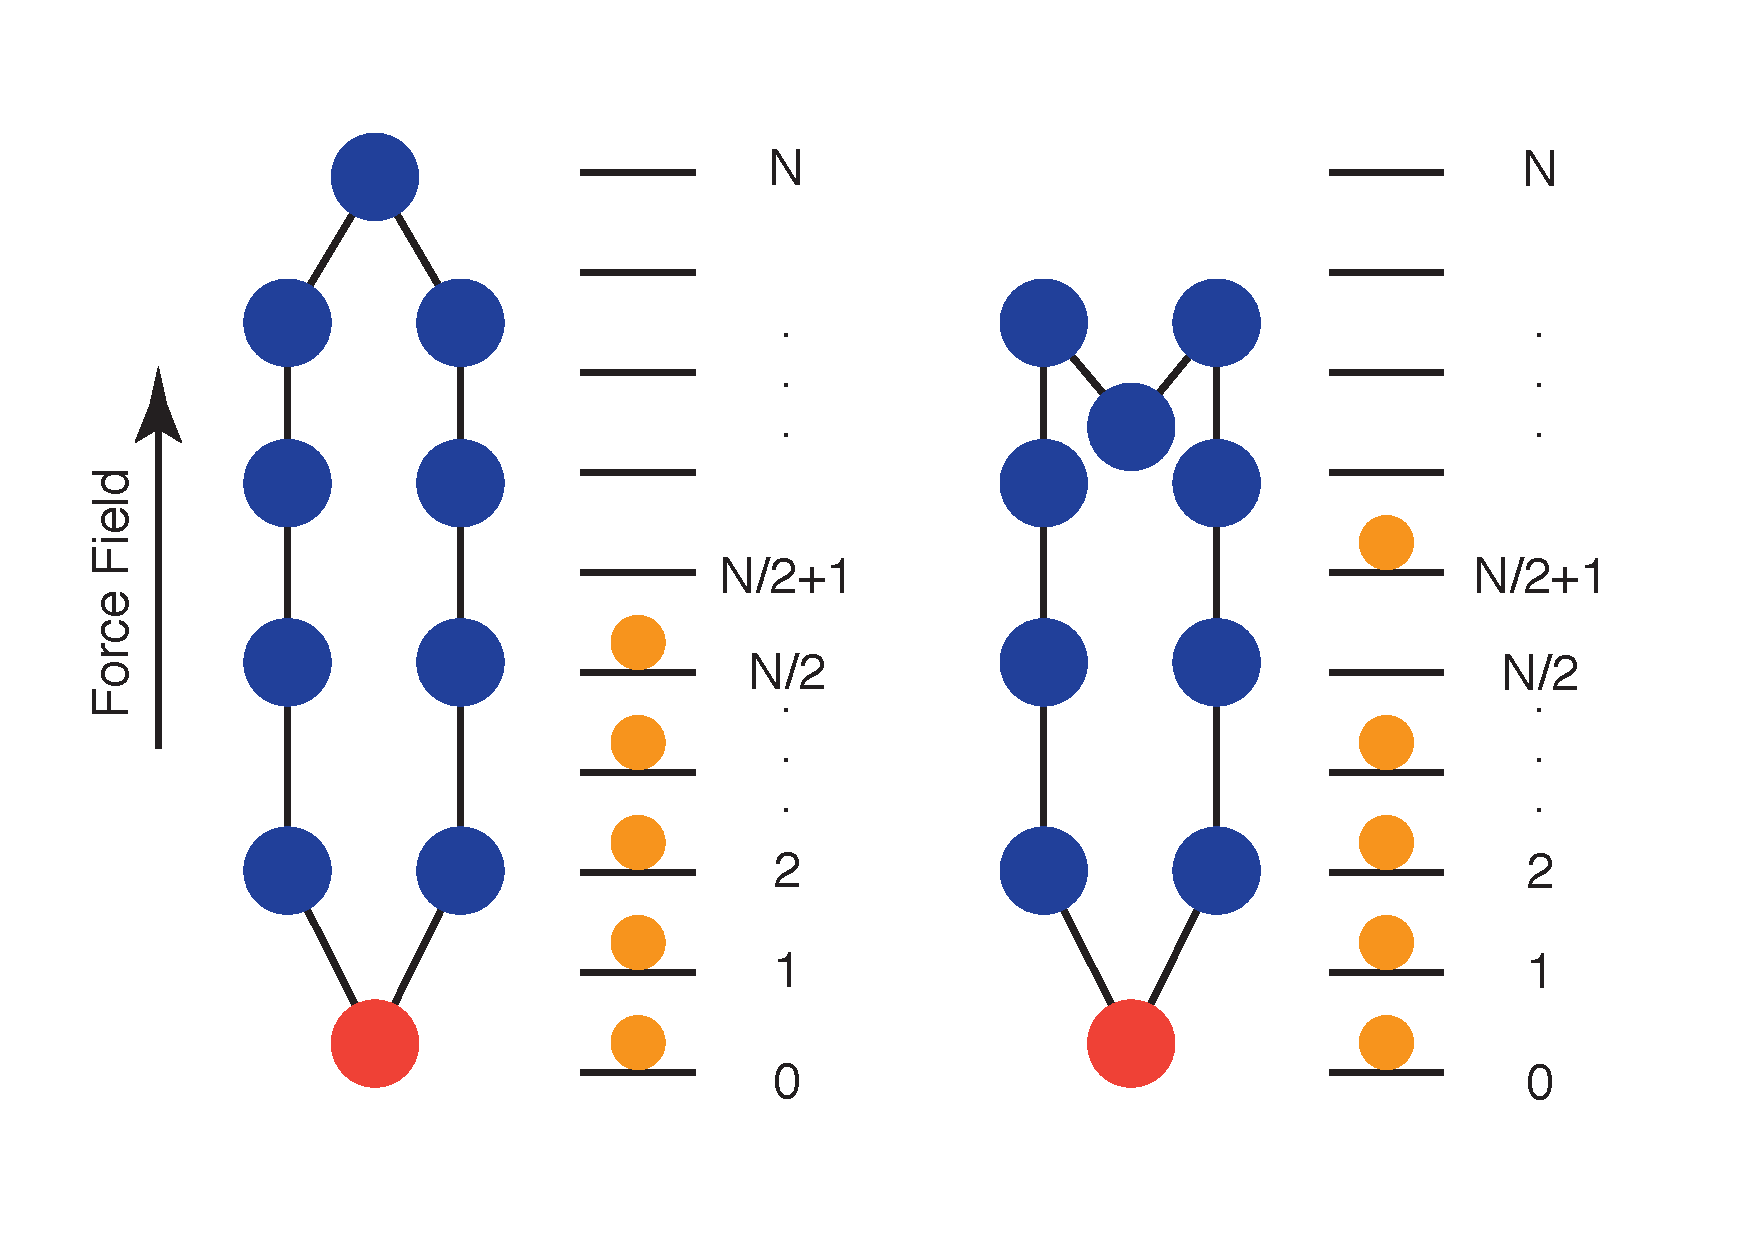
\includegraphics[width=0.8\linewidth]{figureS1}
	\caption{Sketch for analogy of 1D polymer loop to Fermions system.
		Ground state and its corresponding on the left and the first 
		excitation state on the right.}
	\label{fig:s1}
\end{figure}

$N/2$ Fermions are filled in $N$ energy levels. One occupying state of Fermion
system can exactly map to one polymer conformation. Standard Metropolis
scheme\cite{binder2010monte} was exploited to do the sampling. More specifically,
the simulation contains the following steps:

Step 1: initializing the system with the ground state, i.e. all Fermions sit on 
the lower half $N$ energy level. 

Step 2: randomly select a particle and perform a jumping trial to the empty
slot with the probability $p = min\{1,exp\{-(U_{new}-U_{old})/k_B \tilde T\}\}$.
Here $\tilde T$ is the dimensionless temperature defined in the main text. 
$k_B$ is Boltzmann constant. $U_{new}, U_{old}$ is the energy potential of new
and old occupying state which can be calculated
\begin{equation}
	U =  -2 \gamma a v_0\sum_{i=1}^N{jn_j}  
\end{equation}
where $n_j=1$ if the $j$th energy level is occupied and $n_j=0$ if not. 

Step 3: repeat step 2 for enough steps to thermalize the system until it is
equilibrated.

Step 4: sampling the system and transfer it to the polymer configuration scheme
to do the statistical analysis for the average and variance of bead position.

Basically, $10^4$ independent samples after enough thermalization steps are utilized
to collect the statistical results.



\subsection{Brownian Dynamics Simulation}
\label{sub:BDS}
To control the number of free parameters, we choose the ideal bead-rod polymer model to describe the dynamics of chromosomes in nucleus, without considering the exclusive volume effect. 
As we will see later that the system can be reduced to a one free parameter model, i.e. $\tilde{T}$. 

The simulation of model bead connected with rigid rod utilize the technique of Brownian Dynamics\cite{Cruz2012}.
The dynamical equation of beads representing chromosome segments is
\begin{equation}
	\label{eq:differential}
	\dot{\mathbf{r}_i} = \frac{1}{\xi}(\mathbf{F}_i^b + \mathbf{F}_i^c + \mathbf{F}_i^e + \mathbf{F}_i^{pseudo}) 
\end{equation}
where $\mathbf{r}_i$ is the position vector of the $i^{\text{th}}$ bead, $\xi$ is friction coefficient, $\mathbf{F}_i^b$ is random force, $\mathbf{F}_i^c$ is constraint force caused by rigid rod constraints and $\mathbf{F}_i^e$ is external force.
$\mathbf{F}_i^{pseudo}$ is pseudo force added to ensure the right
statistics~\cite{Hinch1994,Cruz2012}.

The random force, which characterizes the fluctuation origin of beads dynamics, is a standard Brownian force which satisfies the following conditions
\begin{subequations}
	\begin{align}
		\left\langle\mathbf{F}_i^b\right\rangle=& \mathbf{0}, \\
		\left\langle\mathbf{F}_i^b (t)\mathbf{F}_j^b (t^{\prime}) \right\rangle=&2k_B T_{c} \xi\delta_{ij}\delta(t-t^{\prime})
	\end{align}
\end{subequations}

$k_B$ is Boltzmann constant and $T_{c}$ is the \emph{characterizing temperature} which characterize the level of randomness arise from the thermal motion of solvent molecules and other interactions between the chromosome and proteins in the nucleus.

The constraint force for a specific bead in a bead-rod ring is
\begin{equation}
	\mathbf{F}_i^c = \lambda_i \mathbf{u}_i - \lambda_{i-1} \mathbf{u}_{i-1}
\end{equation}
where $\lambda_i$ is strength of tension on the rod between $i^{\text{th}}$ and $(i+1)^{\text{th}}$ bead, $\mathbf{u}_i$ is the unit vector along this rod and $\mathbf{u}_{N}$ connects $N^{\text{th}}$ bead and the $1^{\text{th}}$ bead. 

In case of constant force field, the external force is constant $\mathbf{F}_i^e = -\xi \mathbf{v}$ acting on every bead except for the pinned one representing the SPB. 

The pseudo force is calculated using
\begin{equation}
	\mathbf{F}_i^{pseudo} = -\frac{\partial U_{met}}{\partial\mathbf{r}_i};
	U_{met} = \frac{1}{2}k_B T_c \ln(\det \mathbf{G})
\end{equation}
where $\mathbf{G}$ is the metric matrix of the bead-rod system\cite{Pasquali2002}.

Since the rods present in our model are rigid rods, additional constrained equations are needed to keep the rod length unchangeable
\begin{equation}
	\label{eq:constraint}
	(\mathbf{r}_{i+1} - \mathbf{r}_{i})^2 - a^2 = 0
\end{equation}
where $a$ is rod length. 

Dimensionless variables can be obtained by rescaling the parameters $\mathbf{r}^{\prime}\to \mathbf{r}/a$, $t^{\prime}\to t/(\xi a^2/k_BT_c)$, and $\mathbf{F}^{\prime}\to\mathbf{F}/(k_BT_c/a)$. The only free parameter left in the model is the dimensionless temperature $\tilde{T}$, prescribed by 
\begin{equation}
	\label{eq:Teff}
	\tilde{T} = \frac{k_BT_c}{Fa} = \frac{k_B T_c}{\xi v a}
\end{equation}
Numerical scheme employed to solved the set of constrained differential equations (\ref{eq:differential}) and (\ref{eq:constraint}) is the predictor-corrector algorithm, which is used widely in bead-rod simulations\cite{Cruz2012,Somasi2002,Liu1989}.
Basic steps include calculating a prediction of $\mathbf{r}_i(t+\delta t)$ without considering the constraint force followed by a correction step, i.e.\ solving the algebra constraint equations to get constraint forces and re-plugin to the original equations for the corrected $\mathbf{r}_i(t+\delta t)$.
The differential equations are solved using Euler iterative method with a time
step $\delta t = 10^{-4}$.  Statistical results are all obtained based on the
ensemble of no less than $10^{9}$ steps after equilibrium.  


% \bibliography{sm}

\bibliographystyle{plain}
\begin{thebibliography}{1}

\bibitem{binder2010monte}
Kurt Binder and Dieter Heermann.
\newblock {\em Monte Carlo simulation in statistical physics: an introduction}.
\newblock Springer Science \& Business Media, 2010.

\bibitem{Cruz2012}
C.~Cruz, F.~Chinesta, and G.~R\'{e}gnier.
\newblock {Review on the Brownian Dynamics Simulation of Bead-Rod-Spring Models
  Encountered in Computational Rheology}.
\newblock {\em Archives of Computational Methods in Engineering},
  19(2):227--259, May 2012.

\bibitem{Hinch1994}
EJ~Hinch.
\newblock {Brownian motion with stiff bonds and rigid constraints}.
\newblock {\em Journal of Fluid Mechanics}, pages 219--234, 1994.

\bibitem{Liu1989}
Tony~W. Liu.
\newblock {Flexible polymer chain dynamics and rheological properties in steady
  flows}.
\newblock {\em The Journal of Chemical Physics}, 90(10):5826, 1989.

\bibitem{Pasquali2002}
Matteo Pasquali, David~C Morse, and Brownian Dynamics.
\newblock {An efficient algorithm for metric correction forces in simulations
  of linear polymers with constrained bond lengths}.
\newblock 116(5), 2002.

\bibitem{Somasi2002}
Madan Somasi, Bamin Khomami, Nathanael~J. Woo, Joe~S. Hur, and Eric~S.G.
  Shaqfeh.
\newblock {Brownian dynamics simulations of bead-rod and bead-spring chains:
  numerical algorithms and coarse-graining issues}.
\newblock {\em Journal of Non-Newtonian Fluid Mechanics}, 108(1-3):227--255,
  December 2002.

\end{thebibliography}

\end{document}
